%%%%%%%%%%%%%%%%%%%%%%%%%%%%%%%%%%%%%%%%%%%%%%%%%%%%%%%%%%%%
% 文件:     f:\CUSTPaper\test.tex
% 项目:     f:\CUSTPaper
% 创建时间: Thursday, April 25th 2019, 12:27:01 am
% 创作者: ElonH
% --------------------
% 最后修改时间: Sun May 19 2019
% 修改者: ElonH
% ----------------------------------------
% MIT License
% 
% Copyright (c) 2019 ElonH
% 
% Permission is hereby granted, free of charge, to any person obtaining a copy of
% this software and associated documentation files (the "Software"), to deal in
% the Software without restriction, including without limitation the rights to
% use, copy, modify, merge, publish, distribute, sublicense, and/or sell copies
% of the Software, and to permit persons to whom the Software is furnished to do
% so, subject to the following conditions:
% 
% The above copyright notice and this permission notice shall be included in all
% copies or substantial portions of the Software.
% 
% THE SOFTWARE IS PROVIDED "AS IS", WITHOUT WARRANTY OF ANY KIND, EXPRESS OR
% IMPLIED, INCLUDING BUT NOT LIMITED TO THE WARRANTIES OF MERCHANTABILITY,
% FITNESS FOR A PARTICULAR PURPOSE AND NONINFRINGEMENT. IN NO EVENT SHALL THE
% AUTHORS OR COPYRIGHT HOLDERS BE LIABLE FOR ANY CLAIM, DAMAGES OR OTHER
% LIABILITY, WHETHER IN AN ACTION OF CONTRACT, TORT OR OTHERWISE, ARISING FROM,
% OUT OF OR IN CONNECTION WITH THE SOFTWARE OR THE USE OR OTHER DEALINGS IN THE
% SOFTWARE.
% ----------------------------------------
% 更改日志:
% 日期       	说明
% -----------	------------------------------------
% 2019/05/19	附录公式引用格式
% 2019/05/10	多引用
%%%%%%%%%%%%%%%%%%%%%%%%%%%%%%%%%%%%%%%%%%%%%%%%%%%%%%%%%%%%


\documentclass{CustGraduPaper}
\usepackage{lipsum}
\usepackage{bm}

\begin{document}
\cntitle{毕业论文中文题目}
\entitle{The Subject of Graduation Project}
\author{姓名}
\department{专业}
\stunum{23333}
\instructor{指导老师}
\academy{学院}
% \date{时间} %默认当前年份和月份
\makecover
\makestatement

\begin{cnabstract}{关键词1\quad 关键词2}%关键词用\quad
	这是一篇长春理工大学本科生毕业论文\LaTeX 模板?

	这是一篇长春理工大学本科生毕业论文\LaTeX 模板.

	这真的是一篇长春理工大学本科生毕业论文\LaTeX 模板?

	这确实是一篇长春理工大学本科生毕业论文\LaTeX 模板.
\end{cnabstract}
\begin{enabstract}{Word1;~Word2;~Word3;}
	\lipsum[1]

	\lipsum[2]

	\lipsum[3]
\end{enabstract}


\makecontents % or \tableofcontents
\chapter{第一章标题}
这是小四号的正文字体,段间距1.5倍

通过空一行实现段落换行,仅仅是回车并不会产生新的段落
\par 也可以通过\verb|\par|命令来新起一段
\section{第一小节}
\subsection{第一小小节}
\subsubsection{第一小小小节}
\subsection{第二小小节}
\subsubsection{第二小小小节}\label{subsubsubsec:subsubsubsec}

\subsubsection{第四级标题}

\paragraph{段落}\label{para:para}这是一个带有顶头标签的段落这是一个带有顶头标签的段落这是一个带有顶头标签的段落这是一个带有顶头标签的段落这是一个带有顶头标签的段落这是一个带有顶头标签的段落这是一个带有顶头标签的段落
\subparagraph{小段落}\label{subpara:subpara}只是一个带有缩进标签的段落只是一个带有缩进标签的段落只是一个带有缩进标签的段落只是一个带有缩进标签的段落只是一个带有缩进标签的段落只是一个带有缩进标签的段落只是一个带有缩进标签的段落
\section{第二小节}
本模板已经引入伪加粗和伪斜体,这样就不需要对应的粗体和斜体字体也能生成需要的效果,就像下面这样

{\songti \bfseries 宋体加粗}

{\songti \itshape 宋体斜体}

{\songti \bfseries \itshape 宋体粗斜体}

请注意,使用加粗和斜体时,请与字体名称一同使用,否则会自动将粗体匹配为黑体,斜体匹配为楷体,就像下面这样

{正常显示宋体}

{\bfseries 加粗后变为黑体}

{\itshape 斜体后变为楷体}

\section{第三小节}
这是一大段文字这是一大段文字这是一大段文字这是一大段文字这是一大段文字这是一大段文字这是一大段文字这是一大段文字这是一大段文字这是一大段文字这是一大段文字这是一大段文字这是一大段文字这是一大段文字这是一大段文字这是一大段文字这是一大段文字这是一大段文字这是一大段文字这是一大段文字这是一大段文字这是一大段文字这是一大段文字这是一大段文字这是一大段文字这是一大段文字这是一大段文字这是一大段文字这是一大段文字这是一大段文字这是一大段文字这是一大段文字这是一大段文字这是一大段文字这是一大段文字这是一大段文字这是一大段文字这是一大段文字这是一大段文字这是一大段文字这是一大段文字这是一大段文字这是一大段文字这是一大段文字这是一大段文字这是一大段文字这是一大段文字这是一大段文字这是一大段文字这是一大段文字这是一大段文字这是一大段文字这是一大段文字这是一大段文字这是一大段文字这是一大段文字这是一大段文字这是一大段文字这是一大段文字这是一大段文字这是一大段文字这是一大段文字这是一大段文字这是一大段文字这是一大段文字这是一大段文字这是一大段文字这是一大段文字这是一大段文字这是一大段文字这是一大段文字这是一大段文字这是一大段文字这是一大段文字这是一大段文字这是一大段文字这是一大段文字这是一大段文字这是一大段文字这是一大段文字这是一大段文字这是一大段文字这是一大段文字这是一大段文字这是一大段文字这是一大段文字这是一大段文字这是一大段文字这是一大段文字这是一大段文字这是一大段文字这是一大段文字这是一大段文字这是一大段文字这是一大段文字这是一大段文字这是一大段文字这是一大段文字这是一大段文字这是一大段文字这是一大段文字这是一大段文字这是一大段文字这是一大段文字这是一大段文字这是一大段文字这是一大段文字这是一大段文字这是一大段文字这是一大段文字这是一大段文字这是一大段文字这是一大段文字这是一大段文字这是一大段文字这是一大段文字这是一大段文字这是一大段文字这是一大段文字这是一大段文字这是一大段文字这是一大段文字这是一大段文字这是一大段文字这是一大段文字这是一大段文字这是一大段文字这是一大段文字这是一大段文字这是一大段文字这是一大段文字这是一大段文字这是一大段文字这是一大段文字这是一大段文字这是一大段文字这是一大段文字这是一大段文字这是一大段文字
\chapter{新的大节}
新的大节会自动出现在新的一页上
\chapter{参考文献和交叉引用}\label{ch:ref}
\section{参考文献}\label{sec:bibs}
这是一个参考文献引用的范例\cite{Stone_1998},你可以随时使用两种不同的样式\cite{Stone_1998}或者\upcite{Stone_1998}

可以同时引用多个文献\cite{Stone_1998,9780124467422,huagongrenzheng2014}

这样可以添加一个不标注的参考文献引用\nocite{9787508342894}

多引用另一情况\cite{Stone_1998,9780124467422,huagongrenzheng2014,bamboosilk}

这样可以添加所有bib文件中的参考文献\nocite{*}

\subsection{交叉引用}\label{subsec:crossref}
本模板已经重写了hyperref宏包的\verb|\autoref|命令,方便引用章节、公式和图表。

比如说\autoref{ch:ref}、\autoref{sec:bibs}和\autoref{subsec:crossref}就引用了本章节,\autoref{para:para}和\autoref{subpara:subpara}引用了之前的两个段落。显然段落因为没有序号,引用结果和上一节的需要相同,因此建议使用段落“\nameref{para:para}”和段落“\nameref{subpara:subpara}”。

% 本样式定义的第四级标题也可以引用,就像这样:\autoref{subsubsubsec:subsubsubsec}。



\section{公式这么用}
在文中引用公式可以这么写:$a^2+b^2=c^2$这是勾股定理,他还可以表示为$c=\sqrt{a^2+b^2}$,还可以让公式单独一段并且加上编号
\begin{equation}
	\sin^2{\theta}+\cos^2{\theta}=1 \label{eq:pingfanghe}
\end{equation}
还可以通过添加标签在正文中引用公式,如式~\eqref{eq:pingfanghe}~或者\autoref{eq:pingfanghe}。我们还可以轻松打出一个矩阵
\begin{equation}
	\bm{A}=\begin{bmatrix}
		1  & 2  & 3  & 4  \\
		11 & 22 & 33 & 44 \\
	\end{bmatrix}
	\times\begin{bmatrix}
		22 & 24 \\
		32 & 34 \\
		42 & 44 \\
		52 & 54 \\
	\end{bmatrix}
\end{equation}
或者多个带编号的公式
\begin{eqnarray}
	f_1(x)=12x^2+36x+\sin x\\
	f_2(x)=\sqrt{3}{x^3+3x}
\end{eqnarray}
指定某个不带编号
\begin{flalign}
	f(x)=4x^2+5x^2 \nonumber\\
	=9x^2
\end{flalign}
对齐等号
\begin{flalign}
	f(x) & =4x^2+5x^2 \\
	& =9x^2
\end{flalign}
左边大括号
\begin{equation}
	\left\{
	\begin{array}{c}
		f(x)=\frac{log_2(3x^2)}{e^x} \\
		g(x)=\sqrt{3^{2x}}
	\end{array}
	\right.
\end{equation}
来个泰勒公式:
$$
	f(x)=\frac{f\left(x_{0}\right)}{0 !}+\frac{f^{\prime}\left(x_{0}\right)}{1 !}\left(x-x_{0}\right)+\frac{f^{\prime \prime}\left(x_{0}\right)}{2 !}\left(x-x_{0}\right)^{2}+\ldots+\frac{f^{(n)}\left(x_{0}\right)}{n !}\left(x-x_{0}\right)^{n}+R_{n}(x)
$$
Cauchy不等式:
$$
	\left(\int_{E}|f(x) g(x)| \mathrm{d} \mu\right)^{2} \leqslant \int_{E}|f(x)|^{2} \mathrm{d} \mu \int_{E}|g(x)|^{2} \mathrm{d} \mu
$$
麦克斯韦方程组:

\begin{flalign}
	\oint_{S} \mathbf{D} \cdot \mathrm{d} \mathbf{A}& =Q_{f, S} \\
	\oint_{S} \mathbf{B} \cdot \mathrm{d} \mathbf{A}& =0 \\
	\oint_{\partial S} \mathbf{E} \cdot \mathrm{d} \mathbf{l}& =-\frac{\partial \Phi_{B, S}}{\partial t} \\
	\oint_{\partial S} \mathbf{H} \cdot \mathrm{d} \mathbf{l}& =I_{f, s}+\frac{\partial \Phi_{D, S}}{\partial t}
\end{flalign}
对附录中的公式进行引用\autoref{eq:appendices}

以上
\[\frac{123}{2}\]

\chapter{用图和表的示例}
\section{图的使用}
% \XeLaTeX 环境下可以使用EPS、PDF、PNG、JPEG、BMP格式的图片,当然也可以用绘图包直接在\LaTeX 中绘制图形,推荐使用宏包tikz。图的环境是figure,但figure环境使用复杂且不自带标题,因此本模板定义了一个通用版本的generalfig,该环境会将figure内的图片居中并设置标签与引用名,同时会让图片位置设置为所有可行位置(htbp,即此处、页顶、页底、独立一页),此选项可以作为可选参数设置。

其使用方法如下:

\begin{generalfig}[htb]{大数据信息处理框架}{fig:data}
	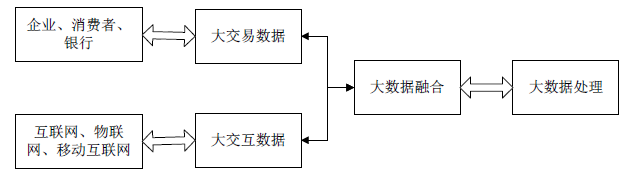
\includegraphics[width=\textwidth]{Figures/data.png}
\end{generalfig}

同时也可以引用该图片例如:\autoref{fig:data}。请注意generalfig第一个参数是标题,第二个参数是引用。

\newpage

\section{表的使用}
作为论文,推荐使用三线表进行排版。所谓三线表,即在标题前有横线,标题后有横线,表格最后还有横线,其他地方无线。当然这不是死规定,也可以根据需要在合适的地方加线。

本文定义了新的可变长度左中右(LCR)格式,LCR三个格式会根据表格宽度的设定自行控制宽度,且其宽度相等,方便设置和页面相同宽度的表格。但该功能需要使用tabularx做表。
\begin{generaltab}{某校学生升高体重样本}{tab:heightweight}
	\begin{tabularx}{\textwidth}{lCCC}
		\toprule
		序号 & 年龄 & 身高   & 体重  \\
		\midrule
		1    & 14   & 156    & 42    \\
		2    & 16   & 158    & 45    \\
		3    & 14   & 162    & 48    \\
		4    & 15   & 163    & 50    \\
		\cmidrule{2-4} %添加2-4列的中线
		平均 & 15   & 159.75 & 46.25 \\
		\bottomrule
	\end{tabularx}
\end{generaltab}

当然你也可以引用表格,就像这样:\autoref{tab:heightweight}。

\section{列表的使用}
这是一个计数的列表
\begin{enumerate}
	\item 第一项
	      \begin{enumerate}
		      \item 第一项中的第一项
		      \item 第一项中的第二项
	      \end{enumerate}
	\item 第二项
	\item 第三项
\end{enumerate}

这是一个不计数的列表
\begin{itemize}
	\item 第一项
	      \begin{itemize}
		      \item 第一项中的第一项
		      \item 第一项中的第二项
	      \end{itemize}
	\item 第二项
	\item 第三项
\end{itemize}

\begin{thankpage}
	感谢老师感谢老师感谢老师感谢老师感谢老师感谢老师感谢老师感谢老师感谢老师感谢老师感谢老师感谢老师感谢老师感谢老师感谢老师感谢老师感谢老师感谢老师感谢老师感谢老师感谢老师感谢老师感谢老师感谢老师感谢老师感谢老师感谢老师感谢老师感谢老师感谢老师感谢老师感谢老师感谢老师感谢老师感谢老师感谢老师

	感谢老师感谢老师感谢老师感谢老师感谢老师感谢老师感谢老师感谢老师感谢老师感谢老师感谢老师感谢老师感谢老师感谢老师感谢老师感谢老师感谢老师感谢老师感谢老师感谢老师感谢老师感谢老师感谢老师感谢老师感谢老师感谢老师
\end{thankpage}

%生成参考文献
%使用方法:\bibliography{参考文件1文件名, 参考文献2文件名, ...}
\bibliography{Bibs/mybib}

\begin{appendices}
	\chapter{第一个附录}
	这里是附录环境,其中的section、subsection、subsubsection已经变为附录的样式,并且会以这种样式加入目录中
	\section{附录可以有小节}
	\subsection{小小节}
	附录公式引用使用带圈数字
	\begin{equation}\label{eq:appendices}
		\nabla F = (
		\frac{\partial F}{\partial x},
		\frac{\partial F}{\partial y},
		\frac{\partial F}{\partial z})
	\end{equation}
	\subsubsection{附录中也可以有小小节}\label{apxsubsubsec:appendix}
	% \verb|\autoref|无法识别Appendices环境,引用效果和正文一样,如\autoref{apxsubsubsec:appendix}。所以如果引用附录的话,建议直接使用附录~\ref{apxsubsubsec:appendix}~。
\end{appendices}


\end{document}
